\documentclass[gra_conf.tex]{subfiles}
\begin{document}

\begin{figure}[h]
  \centering
  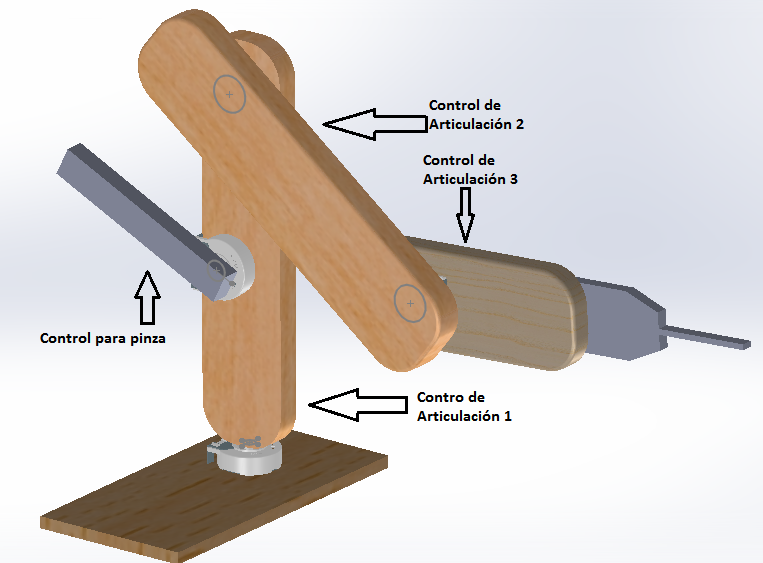
\includegraphics[width=0.3\textwidth]{../img/Replica1.png}
  \caption{Brazo a escala - perspectiva 1}
  \label{brazo_replica1}
\end{figure}

Se puede observar en la imagen 3.1 los sistemas mecánicos para realizar
el control del brazo robótico. En cada articulación se encuentra un 
potenciómetro, el cual cambiará su resistencia en función del ángulo
en el  que se gire cada eslabón. Los eslabones forman una réplica del
brazo robótico, a excepción de la pequeña palanca, la cual funcinará
como control de la pinza.

\begin{figure}[h]
  \centering
  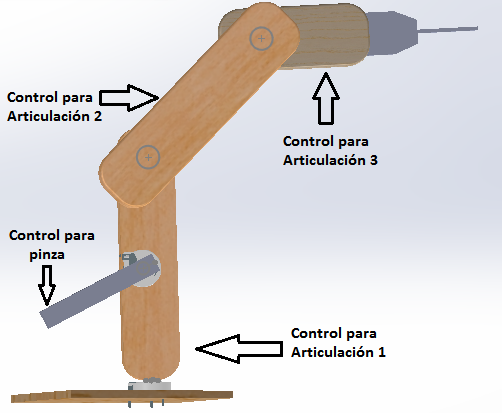
\includegraphics[width=0.3\textwidth]{../img/Replica2.png}
  \caption{Brazo a escala - perspectiva 2}
  \label{brazo_replica2}
\end{figure}

Cada potenciómetro va conectado a una entrada analógica de un Arduino UNO, 
con la cual, junto con un muestreo previo, se podrá aproximar el ángulo del 
potenciómetro, y así, se controlará las articulaciones (1, 2, 3, pinza) del 
robot. Se pueden observar las partes de la réplica en la Fig. 3.2.

\begin{figure}[h]
  \centering
  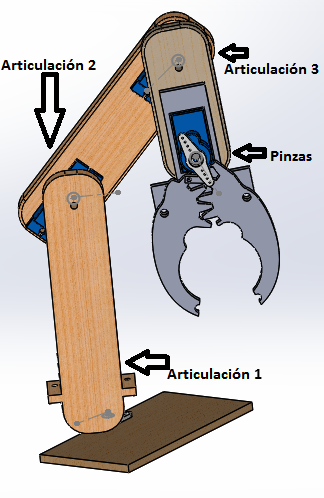
\includegraphics[width=0.2\textwidth]{../img/Brazo1.png}
  \caption{Brazo robótico - perspectiva 1}
  \label{brazo1}
\end{figure}

Se puede observar el chasis del robot en la Fig. 3.3. Cada articulación
tiene $180^\circ$ de amplitud de movimiento en ángulo, debido a que se 
usan servomotores de $90^\circ$.

\begin{figure}[h]
\centering
  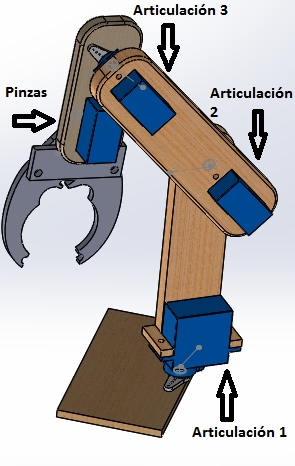
\includegraphics[width=0.2\textwidth]{../img/Brazo2.png}
  \caption{Brazo robótico - perspectiva 2}
  \label{brazo2}
\end{figure}

\end{document}